\documentclass[sigconf,
	anonymous,
%	timestamp,
]{acmart}
\pagestyle{plain}
\settopmatter{printccs=false,printacmref=false}
\renewcommand\footnotetextcopyrightpermission[1]{} % removes footnote with conference information in first column

\usepackage{booktabs} % For formal tables
\usepackage{tikz}
\usepackage{multirow}
\usepackage{amssymb}
\usepackage{url}
\usepackage{amsfonts}
\usepackage{amsmath}
\usepackage{pifont}
\usepackage{enumitem}
\usepackage{hyperref}
\usepackage{tabulary}
\usepackage{mathabx}
\usepackage{stmaryrd}
\usepackage{xspace}
\usepackage{graphicx}
\usepackage[export]{adjustbox}
\usepackage{multirow}
\usepackage{subcaption}
\usepackage{color, colortbl}

\definecolor{Gray}{gray}{0.9}

\newcommand*\rot{\rotatebox{78}}
\newcommand{\saumya}{\textcolor{black}{\ding{51}}}
\newcommand{\xmark}{\textcolor{red}{\ding{55}}}
\newcommand{\note}[1]{\textbf{\textcolor{blue}{[#1]}}}
\newcommand\jason[1]{%
	\textcolor{red}{[\textbf{}
	\ignorespaces #1%
	\ifhmode
		\unskip
	\fi
	]}%
}

\newcommand{\re}{ReCaptcha\xspace}
\newcommand{\system}{AudioBreaker\xspace}
\newcommand{\no}{seven\xspace}

\setlist{leftmargin=2\parindent,
         labelindent=\parindent,
	 labelwidth=*,
	 labelsep*=.5em}

% Print a big black box next to any overfull hboxes.
\overfullrule=5pt

%%%%%%%%command for circles with alphanumeric inside
\definecolor{azure}{RGB}{0,127,255}

\newcommand*\circlea[1]{\protect\tikz[baseline=(char.base)]{
\node[shape=circle, white, font=\sffamily\bfseries, draw=black,
fill=black,inner sep=2pt] (char) {#1};}}

\newcommand*\circleaa[1]{\protect\tikz[baseline=(char.base)]{
\node[shape=circle, white, font=\sffamily\bfseries, draw=black,
fill=black,inner sep=1pt] (char) {#1};}}

\newcommand*\circleb[1]{\protect\tikz[baseline=(char.base)]{
\node[shape=circle, white, font=\sffamily\bfseries, draw=red,
fill=red,inner sep=2pt] (char) {#1};}}

\newcommand*\circlebb[1]{\protect\tikz[baseline=(char.base)]{
\node[shape=circle, white, font=\sffamily\bfseries, draw=red,
fill=red,inner sep=1pt] (char) {#1};}}

\newcommand*\circlec[1]{\protect\tikz[baseline=(char.base)]{
\node[shape=circle, white, font=\sffamily\bfseries, draw=azure,
fill=azure,inner sep=2pt] (char) {#1};}}
%%%%%%%%

%% Copyright
%%\setcopyright{none}
%%\setcopyright{acmcopyright}
%%\setcopyright{acmlicensed}
%\setcopyright{rightsretained}
%%\setcopyright{usgov}
%%\setcopyright{usgovmixed}
%%\setcopyright{cagov}
%%\setcopyright{cagovmixed}
%
%
%% DOI
%\acmDOI{xxx}
%
%% ISBN
%\acmISBN{xxx}
%
%%Conference
%\acmConference[CCS'17]{ACM Symposium on Computer and Communication
%Security}{November 2017}{Dallas, TX, USA} 
%\acmYear{2017}
%\copyrightyear{2017}
%
%\acmPrice{00.00}
%
%\acmSubmissionID{xxx-xxx-xx}
%
\title{In (Cyber)Space Bots Can Hear You: \\ Speech Recognition Attacks Against Audio CAPTCHAs}
%\title{In (Cyber)Space Bots Can Hear You Scream: \\ Breaking Audio Captchas Using Speech Recognition}

% We can actually set the authors now and remove the `anonymous` class option
% above for camera ready.
\author{Anonymous}
\begin{document}

% The new ACM template is dumb. The abstract needs to be defined before the
% \maketitle! See acmart.pdf.
\section{Abstract}\mbox{}\
\label{sec:abstract}

CAPTCHA is a backronym for Completely Automated Public Turing test to tell Computers and Humans Apart. As the name suggests, they are automated tests designed to control access to computer systems by distinguishing humans from bots. Since their launch in 2000, websites have used them extensively to prevent bot account creation and spam. There are many types of tests devised for CAPTCHAS in the past. The most common CAPTCHAS are text based, where an image is shown to the users which contains distorted text. Users are asked to read and recognize this text and type the text they see into a textbox that is situated next to the image. Some other common types of CAPTCHAs include tasks of selecting a single or multiple similar images among many heterogeneous images, solving math puzzles, recognizing 3D text, clicking or dragging moving elements, locating text or numbers in a video, etc. \newline

For a long time now, researchers have tested the strength of text CAPTCHAs and using the latest advancements in computer vision, have been able to break text CAPTCHAs with an accuracy of up to 77\% \cite{ebay:machine-noise}. The version 2 ReCAPTCHA by Google employs checkbox and image CAPTCHAs which again, after scrutiny, have been rendered broken with an accuracy of 70.78\% \cite{recurrent:machine-noise}. Ever since CAPTCHAs have been introduced, companies have built their own CAPTCHA systems and have used them to prevent bot activity on their web pages. Also, a number of enterprise solutions that offer CAPTCHA systems as a service have since emerged. Although CAPTCHAs have become very common, users often encounter CAPTCHAs which are hard even for humans to solve. As there is very less or no margin for error to prevent bot activity, users often end up making multiple attempts to solve a challenge. It has been shown that CAPTCHA challenges frustrate users and it negatively impacts the experience and traffic of a website \cite{distil}.\newline

Commercial CAPTCHA services can be utilized by users by signing up with one of the CAPTCHA providers and including a few lines of their code on the target web pages. ReCAPTCHA is one such service offered by Google. Text and image challenges are the most common CAPTCHAs offered by these services which are implemented on web pages to prevent bots from filling web forms automatically. But a drawback with these CAPTCHA systems is that certain groups of people, especially the visually impaired, find it difficult to use them. Thus, audio challenges were introduced specifically to help computer systems be accessible to the visually impaired. The caveat with this approach is that these audio CAPTCHAs open a new ground for exploitation for attackers.\newline

While there has been a lot of prior work done on breaking text and image CAPTCHAs, audio CAPTCHAs have not been studied to such great detail. In this work, we present a survey of all the audio CAPTCHA services that are currently used and show how we used our system to automate the solving of these challenges using existing, off-the-shelf speech recognition services. We found that the latest version of ReCAPTCHA is very vulnerable to our attack.\newline

  



\maketitle

\section{Introduction}
\label{sec:intro}

\note{First paragraph sets the context.}
While automated attacks continue to plague the Internet, the number
of users from around the world going online has reached unprecedented levels.
Thus, it is crucial to deploy user-friendly mechanisms for preventing bots without
becoming obstacles to legitimate users.

\note{Second paragraph is more specific. Talk about audio captchas, give some relevant statistics.}

According to the World Health Organization 285 million people have some form of visual impairment~\cite{impaired}.

Captchas present an interesting dilemma from a design standpoint, as they are an exemplary instance 
of usability and security being at direct contradiction. Adding more noise (or distortion) to combat 
automated solvers will also have a significant negative effect on the ability of users to actually
solve challenges.

Previous work has found that popular audio captchas are more difficult than their visual counterparts,
which was also corroborated by a subsequent systematic evaluation of users' ability to solve various types of
captchas~\cite{captchas-are-hard}.


\note{Third paragraph is about what has been done before, what has changed and what is missing.}

\note{Fourth paragraph talks about what we have done, describes our system.}

In this work, we consider multiple leading CAPTCHA providers which also provide an optional audio 
challenge along with the traditional text or image challenge. To solve these challenges, we consider 
multiple online speech recognition APIs (which we will henceforth refer to as ``solvers'').

\note{Fifth paragraph gives some of our important results.}

Overall, the main contributions of our work are:

\begin{itemize}

\item We present an extensive evaluation of the audio captcha ecosystem, and demonstrate how available services 
can be broken using off-the-shelf speech recognition services.

\item We bla bla bla.

\item We bla bla bla.

\end{itemize}

\section{Background}{}\mbox \
\label{sec:background}

The main idea behind CAPTCHAs is to provide users with a task which only a human can perform, and cannot yet be performed by automated web programs, known as 'bots'. Two-factor authentication is a relatively new mechanism to make sure that the email and phone number of the user is confirmed to authenticate them as real users, although it requires extra effort on the users' part. Text based challenges are still very lucrative and are widely used control mechanisms to prevent automated form filling as they do not require any extra effort in the form of learning, training or access to mobile phones.\newline

Text based challenges evolved over time from being simple fonts embedded in images to cursive, handwritten text. With the evolution of Computer Vision over time, simple challenges proved ineffective in beating bots and the systems were redesigned to use a combination of distorted handwritten text with a lot of noise in the form of background images, skewed lines and using both black and white text. Speech based challenges came soon after their visual counterparts \cite{kochanski2002reverse, chan2003using} and just like advancements in Computer Vision, there have been similar advancements in natural language processing and in speech-to-text conversion. According to Shirali-Shahreza et al.\cite{shirali2011accessibility} three groups of people have trouble with this form of CAPTCHA - Visually impaired, who constitute 2.6\% of the world's population, users with dyslexia, and users suffering from motor impairment diseases like Parkinson's.\newline

Google introduced reCAPTCHA v2.0 in the year 2014, with the tagline 'Easy on humans, tough on bots'. The new version claimed to use an "advanced risk analysis sytem" that eased users' efforts in solving CAPTCHA challenges. As opposed to the garbled text with random digits and words, this version required the user to click in a checkbox or solve challenges with images. This improved the user experience, while solving the same purpose as the text challenges and was seen as a welcome change by users.\newline


\section{System Overview}
\label{sec:system}

\begin{figure}
\centering
\includegraphics[width=\columnwidth]{figures/breaker_arch.pdf}
\caption{Overview of the CaptchaBreaker system.}
\label{fig:breaker}
\end{figure}

Describe our modular system. What components, how they have been implemented, 
how we create modules for each captcha service, and each speech recognition service.


We built a series of selenium bots that loads each service, obtains the audio file from the captcha for solving via the off the shelf voice recognition service. After the data is received it is post processed and specialzed for each serivce 


\subsection{Background on Selenium} 

To create the bot we utilized the browser automation framework known as selenium. This was the tool of our choice as it is hard to detect scraping/botting written utilizing the selenium webdriver and your browser of choice. Selenium communicates with browsers via a special protocol native to each browser and has access to everything loaded for a web site, the JavaScript, the DOM and even the secure cookies. The special protocol is required as  Selenium RC uses generic javascript for browser automation however executing simply generic javascript violates same origin policy. For every website the browser creates a sandbox for the website's javascript, this way the javascript that belongs to one website does not execute on another website that is currently loaded on the browser. (more detail on cross site scripting). To overcome this Selenium acts as an HTTP Proxy server, when we launch the browser through selenium scripts, javascript (Selenium Core) is injected into the browser, all subsequents requests are therefore through Selenium. In essence selenium makes the browser think that the web application is served from Selenium's domain rather than the actual web server hosting our web application.   

Selenium driving the browser from within by sitting in as injected Javascript provides certian limitations which is handled by "WebDriver" an object oriented api, as the Core is limited by the JavaScript sandbox of the browser (Due to same origin policy). The Webdriver, handles the browser from outside the browser. This was the marked difference between Selenium 1.0 and Selenium 2.0 as by being limited by the sandbox and therefore has reduced functional test coverage. 


[graphic of selenium driving browsers with injected javascript]


\subsection{Why Selenium}

\note{Why selenium is better than other botting/scrapers out there --
}

Almost no way to detect the automation except for checking some predefined variables which most websites do not do.

\note{source : https://stackoverflow.com/a/41220267
}

Web Driver is the nearest you can get to an actual person driving the browser automation. Quote:  "Driving a browser natively as a user would either locally or on a remote machine using the Selenium Server it marks a leap forward in terms of browser automation."

\note{source: http://www.seleniumhq.org/projects/webdriver/
}

\note{need better ways to say this}


We utilized three different voice recognition services for our system, the python google cloud speech api, the ibm bluemix, Wit ai voice recognition services.

\section{Audio Captcha Services}
\label{sec:services}

Describe all the services we will break in the paper. Describe vocabulary, level/type of noise,
system component implementation details (how is the captcha presented, what page elements are handled etc).

\subsection{Recaptcha by Google}

Google's Recaptcha system is the most widely deployed captcha system, which is continuously tweaked to 
adapt to publicized attacks. During our experiments there was a significant change in the audio challenges,
and we will differentiate between the 2 versions in the remainder of the paper.

%Google provides a demo page for Recaptcha, its state-of-the-art captcha system (the version 2 of Recaptcha), 
%accessible via the following URL (https://www.google.com/\newline recaptcha/api2/demo), for anyone who wants 
%to try out the new captcha system. We used this demo page for all our tests on Recaptcha. The page connects 
%over HTTPS and does not require a login. The page initially loads a widget with a checkbox, which on clicking, 
%shows another widget with the image captcha that loads in a new iframe. The audio captcha challenge appears only 
%after clicking on the headphones-like icon in the bottom of the second widget.

\textbf{Recaptcha 2a.}
The audio challenge provided by the recaptcha system spells out 5 digits (the system has now been updated with 
10 digits) consecutively with little or noise, which the user must then identify and enter into the textbox provided. 
The interval between the digits is not a constant value. Each digit may be spelled out by the same person or different 
persons, male or female. Accents do not generally differ to a large extent.

The challenge also provides an option for the user to download the .mp3 version of the audio. The recaptcha system provides 
a margin for error and allows up to 2 incorrect digits out of the 5. We demonstrate how this high margin for error can be 
leveraged to get an almost 100\% accuracy value. We were able to exploit a security flaw in this system that allowed us to 
bypass the rate limiting that was in place.

The recaptcha demo page generates a new captcha challenge each time we connect to it. It behaves exactly like the recaptcha 
v2 widget that is embedded in popular websites such as Quora, BusinessInsider, Twitter, Ticketmaster and many more, as part 
of their account creation process. This was one of the main reasons why we chose to do our tests with the demo page, instead 
of any particular website that employs Google's recaptcha. Our results would thus stay valid on any website that has the latest 
recaptcha widget embedded.

\textbf{Recaptcha 2b.} The latest version of Recaptcha (as of early 2017) is known as the invisible Recaptcha 
(accessible via the following URL https://www.google.com/recaptcha/api2/\newline demo?invisible=true). This 
version does not have an explicit checkbox as seen in the previous version. It relies heavily on the number 
of requests generated per IP address, cookies and other parameters rather than the text/audio challenge itself. 
If the system does not suspect bot activity, it automatically authenticates the user as real even without presenting 
the user with a challenge (i.e. without any user interaction). However, a challenge is presented when the system 
suspects bot activity, and this challenge is very similar to the previous version with respect to the look and feel.

When accessed from a private browsing session, as there are no cookies, the system is suspicious and requires a challenge 
to be solved. This version spells out 10 digits in its audio challenge consecutively with little or no noise at all, with 
an error margin of 1 digit and also allows downloading of the MP3 file from the interface itself. Although we were very 
easily able to transcribe the digits of the audio, we were unable to bypass the rate-limiting that has been set by the system.

\textbf{Recaptcha 1.0} Although still used in many websites, Google has discontinued this version of Recaptcha since 2014. 
Signing up for Recaptcha now enables the newer version by default. It must be
noted that the websites that used this version previously did not automatically upgrade to the No 
captcha Recaptcha version, and they remain open to the vulnerabilities that were fixed in the subsequent 
version. We have obtained \note{X} samples from the authors of prior work~\cite{meutzner2014using} so as to 
compare the effectiveness of our attack that users off-the-shelf speech recognition systems against previous 
studies that trained their own machine learning classifiers.

There are 10 digits that are spoken in the audio challenge and there is very little or no noise. This 
version does not enforce any rate limiting unlike the newer versions of Recaptcha. The margin for error 
is again 1 out of the 10 spoken digits. With respect to the text based challenge, there are two words 
shown which must be recognized by the user and typed into the input field. The first word is an unknown 
text from a failed OCR scan while digitizing physical books and other printed material, and the other 
being a ``control'' word, which is known. This helped transcribe the unknown words and digitize them, and 
in 2012, photographs of house numbers taken from Google's Street View project began to be used, in 
addition to scanned words. 

\subsection{Securimage}

Securimage is an open source captcha system that was developed by Drew Phillips that has 
been under active development and maintenance since 2005. It also has plugins/modules for 
major content management systems like Drupal, Wordpress, Joomla!, etc. It is written in PHP 
and offers very easy integration with websites written in PHP with a lot of customization 
options for both image and audio based challenges. The demo page contains 3 different forms 
of challenges - a random digit/character combination, a math puzzle and a custom captcha 
made from a word list. The demo page can be found here: https://www.phpcaptcha.org/
try-securimage/.

For each audio challenge, the system generates a WAV file from a corpus of audio files of 26 
alphabets (A-Z) and 10 digits (0-9). The digits and alphabets are spoken by only one person. 
The audio is generated by picking 6 word/digit files at random, combining them and adding one 
of the 5 noise files. The default number of digits/characters per challenge is 6, but this can 
be customized while implementing the library. Some other customization options are that one can 
specify a word list for the challenges and using a read-aloud math puzzle that is to be solved 
by the user. Securimage does not offer any margin for error.

\subsection{Captchas.net}

Captchas.net, started back in 2004 offers implementation and easy integration for PHP, ASP, Perl, 
Python, JSP and Ruby. It is a free service, but shows a watermark on the images of the text challenges 
which can be removed by subscribing to the paid version. For both the text and the audio challenges, 
Captchas.net follows the following method to validate the response:

\begin{itemize}
\item Both the client server and Captchas.net's server share a common secret key.
\item The secret key and a random string sent by the client are used to generate the password.
\item The password is computed by Captchas.net's server to generate the image and by the client server to validate the user's input.
\end{itemize}

The text challenges always consist only of alphabets and the audio challenge uses NATO alphabets 
of the same text challenge. For instance, ``RIPAZH'' would be read out as 'Romeo, India, Papa, Alpha, 
Zulu, Hotel' and the user is expected to enter the first letter of each uttered word. There is no 
margin for error in this service and there is little background noise.

\subsection{Apple}

Apple's captcha is encountered while signing up for a new iCloud account 
Before spelling out the audio challenge, 
the voice first says ``Please enter the $n$ numbers that you hear in the textbox provided''. The 
spoken numbers consist of two digits like 25, 64, etc. and they are always spoken by a single person. 
The page times out after two minutes of inactivity and a pop up appears for confirmation if the user is 
still in the process of creating the account. Apple does not allow downloading the audio file and is 
loaded and played via JavaScript and not stored in any cache or temporary storage.

To obtain the audio file for the challenge, one has to manually open the URL chrome://media-internals 
on the Google Chrome browser. The Media Internals feature of Chrome displays three things \cite{media}:
\begin{itemize}
\item Everything it can dig up from the media stack about active media players. Includes buffered data, 
    video properties, measured times between events, and a log of events.
\item Status and volume of active audio streams. These are not yet associated with a particular tab.
\item Cache activity, including reads from and writes to the media cache.\newline
\end{itemize}

\subsection{RadCaptcha by Telerik}

RadCaptcha is a captcha service by Telerik that is built especially for ASP.NET 
web applications. RadCaptcha and 90+ other controls are part of UI for ASP.NET AJAX, 
a comprehensive toolset that take care of the common functionality of a ASP based 
CMS like Sitefinity \cite{radcaptcha}. It is also a part of a feedback form for the 
HR website of UIC, where we discovered this captcha. It can be seen here: https://www
.hr.uic.edu/cms/One.aspx?pageId=356957\newline

RadCaptcha's audio challenge speaks out digits (0-9) and alphabets in NATO form. It is 
spelt out by a single speaker and there is almost no background noise in the audio. The 
audio is not available to download explicitly, but is present on the DOM of the web page 
in an <audio> tag, from which the URL of the audio file can be easily grabbed. One of the 
customizations provided by the service is a rate limit system, which requires the form to 
be displayed to the user for a particular number of seconds before it can be considered as 
human-submitted. However, this setting is left to the person who implements the captcha 
service on the web page.

\subsection{BotDetect}

BotDetect offers free and paid versions of its captcha system. In the free version, the 
service has several limitations, like the audio challenge is not fully functional most of 
the times. There is a 50\% chance that the audio challenge is replaced with an audio file 
that speaks "Sound Demo". BotDetect offers libraries for integration with .NET, Java, ASP 
and PHP based websites. The demo page of BotDetect can be accessed here: 
\url{https://captcha.com/demos/features/captcha-demo.aspx}.

The audio challenge speaks out exactly the digits and characters in the text/image challenge. 
While implementing the captcha service on one's website, the web master has a lot of customization 
options. For instance, the number of alphanumeric characters in the challenge can be chosen between 
1-13 (the default being a random of 4-6). The background noise can be random or selected from one of 
the 10 noise types and the sound type can be customized as well (choice of 8 Bit Mono audio or 16 Bit 
Mono audio). We found that this service is used widely, and we encountered it on the Visa status check 
page of US CEAC website here: https://ceac.state.gov/ceacstattracker/status.aspx \newline

\subsection{Live.com}

Live.com, owned by Microsoft is a service that provides access to other Microsoft services. 
Some of these are Windows, Microsoft Store, OneDrive, Bing, MSN, Office, Skype, Outlook.com, 
Xbox Live, etc. The captcha is encountered while registering for a new account with Live.com 
at \url{https://signup.live.com}.

The audio challenge of Live.com speaks out random words from the English vocabulary. On average, 
they are 5 letter words and 5-7 such words are spoken per challenge, which must be typed by the user. 
The words are spoken by 2 different people - one female and one male, although we found that the number 
of words spoken out by the female voice are much higher. In our opinion, it provided better accessibility 
to visually impaired users as they can press '1' on their keyboard to play or repeat the audio challenge 
and by requesting a new challenge using the button labeled 'New' on the interface, the focus is set to the 
response box automatically.

\begin{table*}[h]
\centering
\caption{Accuracy of different speech recognition services and accents against the audio captcha services we evaluated.}
\begin{tabular}{lccccc}
\toprule
&\multicolumn{5}{c}{\textbf{Speech Recognition Service (Accent)}}\\
\cmidrule{2-6}
\textbf{Captcha Service}& \textbf{Wit}& \textbf{IBM (US)} & \textbf{ IBM (UK)} & \textbf{Google (US)} & \textbf{Google (UK)} \\
\hline
Recaptcha v2.0 & 67.1\% (671/1000) & 95.8\% (958/1000) & 67.2\% (672/1000) & \textbf{98.3\%} (983/1000) & 81.6\% (816/1000) \\
\rowcolor{Gray}
Recaptcha v2.1 &  &  &  &  & \\
Apple  & 0\% (0/365)  & 2.3\% (6/260) & 6.8\% (17/251) & 35.8\% (126/352) & \textbf{52.8\%} (143/271) \\
\rowcolor{Gray}
BotDetect  & 1.23\% (11/894)  & 1.38\% (19/138) & 6.67\% (12/180) & \textbf{9.5\%} (102/1067)  & 6.65\% (79/1187) \\
Captchas.net  & 0\% (0/1008) & 1.1\% (9/778)  & 0.3\% (3/1010)  & 2.7\% (16/593) & \textbf{22.3\%} (230/1030) \\
\rowcolor{Gray}
Microsoft Live & &  &  & & \\
Securimage  & 0\% (0/1000)  & 0\% (0/1000) & 0\% (0/1000) & 0.1\% (0/1000) & \textbf{3\%} (30/1000) \\
\rowcolor{Gray}
Telerik  & 21.2\% (142/668)  & \textbf{97\%} (452/466) & 12.9\% (47/364) & 74.2\% (150/202) & 49.3\% (112/217) \\
\bottomrule
\end{tabular}
\label{tab:combinations}
\end{table*}

\section{Experimental Evaluation}
\label{sec:evaluation}

In this section we present the results from our extensive experiments again 
the audio captcha services presented in Section~\ref{sec:services}.

\textbf{Attack accuracy.} Table~\ref{tab:combinations} presents the accuracy obtained by each speech recognition service 
against the audio captcha services. In cases where the speech recognition service has the option to select an accent,
we experiment with both American and British English. Surprisingly, we find that for every single captcha scheme, at least
one of the speech recognition services is able to solve more challenges than the 1\% threshold, thus, \emph{practically 
rendering all captcha schemes broken.} Nonetheless, there is significant variance, not only across captcha schemes, but
the accuracy obtained by each speech recognition engine for a specific captcha service. 

The most alarming finding is 
that \system achieved the highest accuracy against \re v2.0, the most widely deployed captcha service. When compared 
to the 70.78\% attack accuracy reported for the image \re~\cite{sivakorn:eurosp16}, it becomes apparent that audio challenges
weaken the overall security offered by \re, as fraudsters can target audio captchas for deploying highly successful
attacks. The Apple and Microsoft Live captchas that protect their account creation process, are also highly susceptible to 
automated attacks, as our approach correctly solves up to \note{52.8\% and X\%} respectively.

Despite the presence of noise impacting the accuracy of the transcription process for all the respective captcha schemes
(see Table~\ref{tab:services}), none of the services is completely impervious to our attacks. Nonetheless, we
found that the audio captchas from Securimage are the most robust due to the presence of background semantic noise,
as \system was only able to solve 3\% of the challenges when using Google's Speech API and the British English accent
configuration. Another interesting observation was that no single speech recognition system or configuration
was consistently more accurate across all captchas; however, Google's speech recognition achieved the best
results for \note{X} out of the \note{Y} captcha schemes. While attackers could increase the attacks' accuracy
by first pre-processing the audio challenges so as to reduce the noise, the motivation behind our study is to 
demonstrate how attackers can employ off-the-shelf systems for breaking existing captcha systems.
Based on these results, we find that \system would be an effective replacement to the human solvers employed by
captcha solving services, as humans are often troubled by audio captchas~\cite{captchas-are-hard}.


\begin{table}[t]
\centering
\caption{Average solution time for each recognition service and accent against the audio captcha services we evaluated.}
\begin{tabular}{lccccc}
\toprule
&\multicolumn{5}{c}{\textbf{Speech Recognition Service}}\\
\cmidrule{2-6}
& & \textbf{(US)} & \textbf{(UK)} & \textbf{(US)} & \textbf{(UK)} \\
\textbf{Captcha}&  \textbf{Wit} & \textbf{IBM} & \textbf{IBM} & \textbf{Google} & \textbf{Google} \\
\hline
Recaptcha v2.0 & 13.85s & 10.56s  & 12.25s & \textbf{18.46s} & 20.41s \\
\rowcolor{Gray}
Recaptcha v2.1 &  &  &  & & \\
Apple  & 36.4s & 33.4s  & 34.7s & 15.5s & \textbf{13.9s} \\
\rowcolor{Gray}
BotDetect  & 5.53s  & 4.21s & 5.72s & \textbf{3.40s} & 3.05s \\
Captchas.net  & 19.92s  & 14.62s  & 15.65s  & 7.56s & \textbf{7.79s} \\
\rowcolor{Gray}
Microsoft Live & &  &  & & \\
Securimage  & 34.31s & 23.60s & 25.10s  & 27.29s & \textbf{35.28s} \\
\rowcolor{Gray}
Telerik  & 7.53s & \textbf{5.56s} & 6.65s & 3.86s & 3.83s \\
\bottomrule
\end{tabular}
\label{tab:solution_time}
\end{table}

\textbf{Solution time.} In Table~\ref{tab:solution_time} we include the average time required by each speech recognition 
service for returning a transcription of the audio captcha. The bold values denote the combination that achieved the highest 
accuracy for that captcha scheme. \note{Talk about results.}

\note{How many mistakes allowed for a correct answer?}

\textbf{Rate limits and economic analysis.} Our study's goal is to explore the feasibility of low-cost attacks 
against popular captcha services; thus, the scale of such an attack is naturally constrained by the rate
limiting enforced by the speech recognition APIs. While an attacker could build an offline solver
using a deep learning framework like TensorFlow~\cite{abadi2016tensorflow}\footnote{Researchers have already
released prototypes that build on Tenserflow: {https://github.com/mozilla/DeepSpeech}.} to overcome this constraint,
our threat model explicitly includes non-sophisticated attackers that do not develop or train their own 
classifiers. As such, the rate limits of each speech recognition service become relevant as they could
constrain our attacks.

\begin{table}[t]
\centering
\caption{Attacker's estimated daily profit for each captcha service, when using one Google Speech API account
(with the most accurate accent configuration for that captcha scheme).}
\begin{tabular}{lccc}
\toprule
& \textbf{Captcha} & \textbf{Estimated} & \textbf{Daily} \\
\textbf{Captcha}&  \textbf{Duration} & \textbf{Solutions} & \textbf{Profit} \\
\hline
Recaptcha v2.0 & 7 sec & 242,413 & \$485.3 \\
\rowcolor{Gray}
Recaptcha v2.1 & 15 sec & & \\
Apple  & & & \\
\rowcolor{Gray}
BotDetect  & 6 sec & 28,215 & \$54.7 \\
Captchas.net & 14 sec & 27,524 & \$55 \\
\rowcolor{Gray}
Microsoft Live & & & \\
Securimage & 10 sec & 5,184 & \$10.3 \\
\rowcolor{Gray}
Telerik & 7 sec & 188,892 & \$366.3 \\
\bottomrule
\end{tabular}
\label{tab:money}
\end{table}

Surprisingly, these services have very lax limits that would enable fraudsters to misuse
them for maintaining large scale audio captcha solving campaigns. For instance, Google's Speech API allows up
to 250,000 requests per day, where multiple audio files can be submitted per request, allowing for a maximum of
480 hours of audio processing\footnote{https://cloud.google.com/speech/limits}. 
In Table~\ref{tab:money} we provide a rough estimation of the profit that an attacker could yield against 
each captcha service per day using a single Google API account. We assume a lower end market price of \$2 
per 1,000 solved captchas, and calculate the number of solved captchas based on the length of audio challenges 
and the highest accuracy achieved by a Google Speech solver (see Table~\ref{tab:combinations}) for each service.
\note{Most noteworthy results.} It is important to note, however, that these calculations assume that the attacker 
is not constrained by other forms of rate limiting (e.g., IP-based limits). Given the workarounds employed
by existing captcha solving services (e.g., proxies, botnets, etc), in practice these limitations will not 
pose insurmountable obstacles.

On the other hand, IBM Watson allows 1 free month per account\footnote{https://www.ibm.com/watson/services/natural-language-classifier/}.
Finally, Wit does not have an explicit rate limit. However, it is open to commercial
apps and requests notification for rates approaching one request per second. As all three services
only require an email address for creating an account, attackers could trivially register 
new email addresses periodically for increasing their overall allowed throughput.

%In comparison Clarifai,
%the most accurate image annotation service used against \re~\cite{sivakorn:eurosp16}, only allows 5,000
%free operations per month\footnote{https://developer.clarifai.com/pricing/}.


\textbf{Solution flexibility.} \note{How many wrong digits allowed per service?}

\begin{figure*}[t]
\begin{subfigure}{0.75\textwidth}
    \centering
    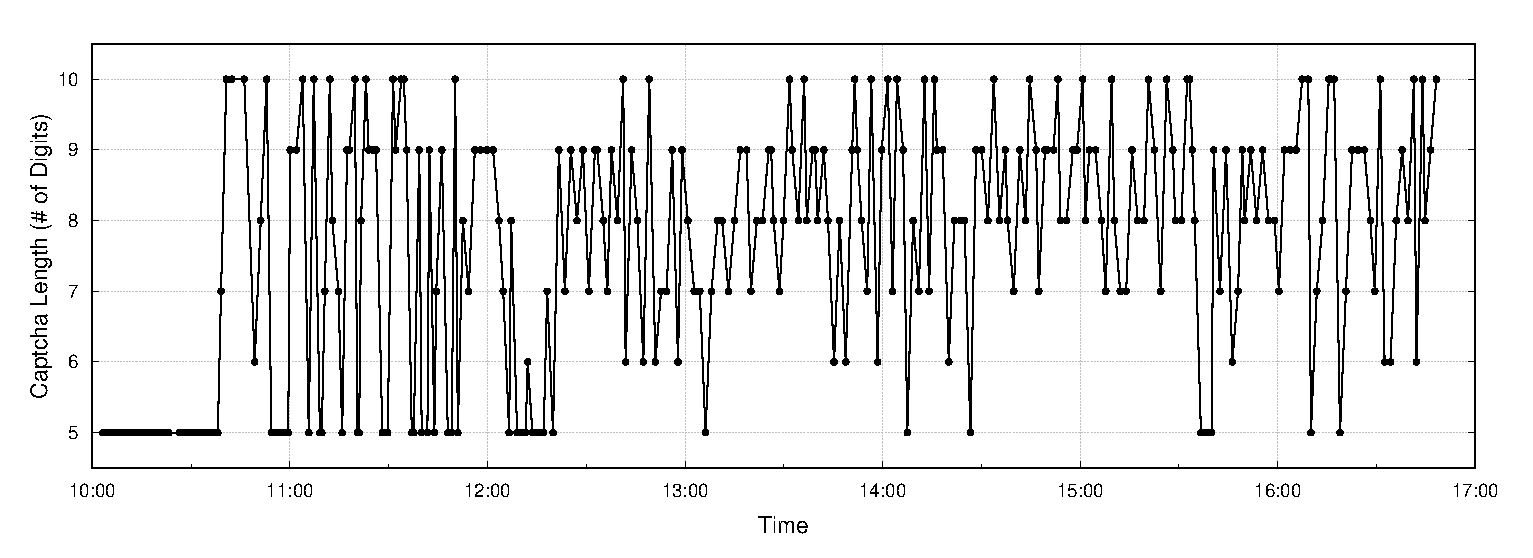
\includegraphics[width=1\textwidth]{figures/captcha_length.eps}
    \label{fig:length_time}
\end{subfigure} %\hspace{0.03\textwidth}
\begin{subfigure}{0.2\textwidth}
    \centering
    %\caption{Average solution time for each recognition service and accent against the audio captcha services we evaluated.}
    \label{tab:length}
    \begin{tabular}{lc}
    \toprule
    \textbf{Digits} & \textbf{\# of Captchas} \\
    \hline
    5 & 95 (31.3\%) \\
    \rowcolor{Gray} 
    6 & 14 (4.6\%) \\
    7 & 34 (11.2\%) \\
    \rowcolor{Gray} 
    8 & 51 (16.8\%) \\
    9 & 68 (22.4\%) \\
    \rowcolor{Gray} 
    10 & 41 (13.5\%)\\
    \bottomrule
    \end{tabular}
\end{subfigure}
\caption{Variation of audio captcha length in \re v2.0 over time.}
\label{fig:length}
\end{figure*}

\textbf{\re.} While our study aims to evaluate the robustness of many popular audio captchas, 
Google's \re is the most prevalent captcha service, so we offer some interesting details 
and findings from our experiments.

\emph{Bypassing rate limits.} As aforementioned in Section~\ref{sec:recaptcha}, \re enforces 
rate limiting to prevent large scale attacks from a small number of machines. While in practice
captcha solving services employ proxies~\cite{captcha_proxies} and botnets (e.g., KoobFace~\cite{captcha_solvers}) 
to overcome such limits, we further explored this mechanism during our experiments. Initially,
we employed a straightforward approach of circulating through a list of valid User Agent strings,
so as to masquerade as numerous computers connecting from a single IP address (e.g., users behind a NAT).
However, in that case \re would enforce the same limit. Surprisingly, though, we found that if we 
supplied a bogus nonsensical User Agent we were able to completely bypass the rate limiting,
and only faced issues when issuing many concurrent solvers (which could be flagged as a potential DDoS attempt).
%solving  well over a thousand captchas per day from a single IP address. 
We surmise that a bug in the risk analysis
system does not enforce the check on the other aspects of the request (e.g., IP address, HTTP cookies) when
it encounters an ``invalid'' User Agent\footnote{This issue has now been fixed.}.
%This incident 
%further highlights how seemingly complex captcha services ]

\emph{Adaptive length}.
While by default the length of \re v2.0 was 5 digits, we found %that after multiple captcha solutions by our system,
that \re would adapt when facing a large amount of requests from our system and return captchas with more digits. 
In Figure~\ref{fig:length} we present a representative experiment that depicts the number of digits in the captchas
processed by our system over the course of 7 hours. The first 49 captchas all contained 5 digits, whereas the length
changed in a seemingly random fashion. As can be seen by the breakdown statistics in the Figure, apart from the default
version with 5 digits, the most common variation we came across contained 9 digits.
%Overall, out of the 303 challenged processed in the experiment, 95 (31.3\%)
%had a length of 5, 14 (4.6\%) had 6 digits, 34 (11.2\%) had 7, 51 (16.8\%) had 8 digits, 68 (22.4\%) had 9, and 41 
%(13.5\%) had 10 digits.

\begin{figure*}[tp]
\begin{subfigure}{0.24\textwidth}
\includegraphics[width=\textwidth]{figures/recaptcha_evolution/2011.pdf}
\caption{\re cca. 2011}
\label{fig:apple}
\end{subfigure} \hspace{0.01\textwidth}
\begin{subfigure}{0.24\textwidth}
\includegraphics[width=\textwidth]{figures/recaptcha_evolution/2014b.pdf}
\caption{\re cca. 2014}
\label{fig:botdetect}
\end{subfigure}\hspace{0.01\textwidth}
\begin{subfigure}{0.24\textwidth}
\includegraphics[width=\textwidth]{figures/recaptcha_evolution/2016.pdf}
\caption{\re cca. 2015-2016}
\label{fig:captchas}
\end{subfigure}
\begin{subfigure}{0.24\textwidth}
\includegraphics[width=\textwidth]{figures/recaptcha_evolution/2017.pdf}
\caption{\re after March 2017}
\label{fig:live}
\end{subfigure}
\caption{The evolution of \re audio challenges through time.}
\label{fig:evolution}
\end{figure*}


\emph{Evolution through time.} In their extensive user study on the usability of captchas, Burzstein et al.~\cite{captchas-are-hard}
found that users were able to solve only 47\% of \re's audio challenges (that number was calculated following an optimistic approach
and is an upper bound to the actual accuracy). Since then \re has modified their audio challenges. % to be more user friendly.
Here we further explore how audio \re has evolved through time. 

In Figure~\ref{fig:evolution} we visualize audio captcha samples
that capture \re's evolution through time. Indeed, the audio challenges from 2011 are the least ``user-friendly'' as they contain
a significant amount of background noise in the form of unintelligible discussions, reversed recordings of speech. While the version
from 2014 is considerably clearer and only five digits long, the audio quality of the spoken digits remains ``noisy'', while background recordings were
also sporadically interjected. In the sample plotted here, a background recording uttering ``three'' is almost overlapping with the
digit spoken as part of the challenge (shown in red). As part of their ``No Captcha Recaptcha'' system released in December 2014, the audio challenges were 
more simplified as they contained five digits with less noise in the recordings; however, certain recordings are processed and the sounds
are more drawn out. This could potentially be a countermeasure against automated attacks. 
Finally, in the current version which was released in March 2017,
the challenges once again contain 10 digits. 

While there might have been more intermediary changes apart from the ones presented here,
this samples show a clear evolution of audio \re challenges towards a more user-friendly scheme. The change in the latest version 
is most likely an attempt to mitigate automated attacks; however, this can only serve as a temporary measure as our experiments
demonstrate that speech recognition technology has reached a point where such challenges can be trivially bypassed. Thus, it remains 
to be seen whether \re adopts an approach similar to services like Securimage and BotDetect and reverts back to challenges with 
more noise and distortion to hinder automated attacks.

\section{Discussion}
\label{sec:discussion}

How can we fix this problem? The amount of noise we can add before an audio captcha becomes unusable is 
far more constrained than for visual challenges.

Human hearing is more error prone than vision~\cite{o2009auditory,shinn2008object}.

\section{Related Work}
\label{sec:related}

\textbf{Breaking audio captchas.} Tam et al.~\cite{tam2008improving} were the 
first to evaluate the robustness of audio captchas against automated attacks,
and reported a success rate of 58\% against audio captchas that contained 
digits and random speech segments as background noise. Subsequently, 
Burzstein and Bethard presented Decaptcha, a system that was able to solve 75\%
of eBay's audio captchas~\cite{Bursztein2009}. While they experimented with Sphynx,
which was at the time a state-of-the-art speech recognizer, they were only able to 
achieve a 1\% accuracy. On the other hand, our experiments reveal how speech recognition
technology has greatly evolved, allowing us to accurately solve audio challenges
across a large number of services.

Bursztein et al.~\cite{bursztein2011failure} conducted an extensive study on audio audio 
challenges that contained digits and letters and broke the Yahoo, Microsoft, and eBay 
captchas with approximate success rates of 45\%, 49\%, and 83\% respectively. However, 
their system was only able to solve $\sim1.5\%$ of \re challenges, due to the presence 
of semantic noise. More recently, Sano et al.~\cite{Sano2013} focused on the \re
version that contained semantic noise and implemented a custom solver that achieved the best
results up to that point, with a 52\% accuracy. Meutzner et al.~\cite{meutzner2014using} demonstrated 
an improvement over those results and reported a 63\% accuracy against the same version of \re. While
we experiment with the latest versions of \re, which have differences, 
we obtain significantly better results with a 83.9\%-98.3\& accuracy.

\textbf{Captchas and accessibility.} According to Shirali-Shahreza et al.~\cite{shirali2011accessibility},
three groups of people have trouble with visual challenges; the visually impaired,
with dyslexia, and users suffering from motor impairment diseases like Parkinson's.
Chellapilla et al.~\cite{Chellapilla} argued that Human-friendly Interaction Proofs (HIPs)
must approach a success rate of at least 90\%. They also argued that, due to their scale, automated attacks
should be able to solve a challenge in less than 0.01\% of their attempts, for a captcha system to be considered
robust. Sauer et al. conducted a usability study with six blind participants on Google's \re, 
and found that they were only able to solve 46\% of the audio challenges~\cite{sauer2008towards}.
They also found that the average amount of time taken to correctly solve an audio challenge was over 65 seconds.
This is significantly higher than the 28.4 seconds that users required for solving audio captchas
in the extensive user study conducted by Bursztein et al.~\cite{captchas-are-hard}.

While conducting a study with blind high school students, Bigham et al.~\cite{bigham2008inspiring}
found that when the students were presented with an audio captcha, none of them were able to solve the challenge 
and their sighted instructors ended up solving the visual version instead. In a subsequent
study conducted with 89 blind users~\cite{bigham2009evaluating}, they found that users achieved 
only a 43\% success rate when solving 10 popular audio captchas.
%In the same study \cite{bigham2009evaluating}, it was also found that screen readers used by blind users speak over
%playing captchas. As users navigate to the answer box, the accessibility software continue speaking the interface while
%talking over the playing audio challenge. A playing audio challenge does not pause for solvers as they type their answer
%and reviewing an audio captcha is cumbersome, often requiring the user to start again from the beginning. Also, replaying
%an audio captcha requires solvers to navigate away from the answer box in order to access the controls of the audio player.
%Thus, the authors proposed a system and optimized the interface of popular audio captcha services without altering the
%underlying implementation and found that the performance increased to 59\%. 

Holman et al.~\cite{holman2007developing} proposed the extension of image captchas to include related
sounds (e.g., an image challenge showing a train would be accompanied by an audio recording of a train), 
as an alternative type of challenge for blind users. An alternative design that required users to identify 
a series of sounds was later proposed~\cite{Lazar:2012}, and the authors conducted a user study in which the
participants achieved a success rate of over 90\%. Krol et al.~\cite{krol2016better} conducted a user study 
to explore a replacement to current captcha schemes but found that users were apprehensive due to the privacy 
concerns as well as an increased sense of frustration.

\textbf{Other applications of audio captchas.} Polakis et al.~\cite{polakis:syssec11} proposed the deployment of 
simple audio challenges (e.g., solving simple math equations, or spelling words with a traditional telephone keypad)
as a defense against automated attacks in telephony systems. Markkola and Lindqvist~\cite{markkola2008accessible}
proposed the deployment of audio captchas that contained digits for preventing telephone SPAM~\cite{sok-robocalls}.

\textbf{Google \re.} In a recent study, Sivakorn et al.~\cite{sivakorn:eurosp16} demonstrated how off-the-shelf 
deep learning systems could be employed for breaking Google's image-based \re system. They also presented a series 
of safeguards employed by \re for preventing automated attacks. Similarly, in our study we demonstrate how off-the-shelf 
speech recognition systems can be used for breaking a wide range of audio captcha systems, and identify a varying set
of safeguards across certain captcha services. Interestingly, our experiments demonstrate a significantly higher success rate,
underlining the importance of finding suitable alternatives for accessible captchas, as the availability of audio captchas 
exposes services to significant risks.


\note{Comparison to low resource attack in w00t paper}

\note{The paper focuses only on Google ReCaptcha and only the second version of it. Unlike this paper our attack focuses on audio captchas from 8 captcha services. It utilizes 6 audio services (Google cloud, bing speech recognition, ibm bluemix, google speech api, wit ai, sphinx) to tackle the google recaptca v2. On the surface level our attack and the one described in the paper may seem similar however there are some important distinctions.} 

\note{Our attack consists of taking the entire audio file and sending it to the cloud services, and with some post processing i.e mapping consistent erroneous transcriptions checking it against the captcha service. Each solver works individually. This allows us to map the errors from each service better as distinct patterns arise per service and cloud speech recognition service. We believe this causes us to get similar rates to the one described in the w00t paper. We also observed variance in performance when each service checks the audio while set to a particular accent. We also observe that they wOOT paper does not run as extensive an evaluation as we do. (From their paper  -- After successfully running against over 450 captchas, it can defeat reCaptcha with over 85% accuracy)
}

\note{The problem statement that they approach is purely for numbers as audio captcha, whereas our attack focuses on alpha-numeric, NATO phonetic spelling, phrases which are dictionary words as well (As said before we attack 8 other services). Like our attack they also apply mappings to improve the efficiency of transcriptions received from each cloud service. They have added different categories for it whereas we lump them as one. They divide them as exact-homophone and a near homophone. They describe an exact homophone as when the word transcribed by the audio service is describing how the number sounds (for example “four” as “for” ) and a near homophone as a slightly erroneous but close enough transcription of the number (for example “six” as “sex”). }


\note{The attack method in the woot paper involves dividing the audio file into its constituent digit audio snippets and then sending those audio snippets to multiple cloud based audio services which send back a number of different valid answers and then utilizing homophone predictions to accurately decide which of those transcriptions are correct, then they assemble the digits from each service based upon a confidence score assigned as per their analysis.}

\note{Our attack method is markedly different from theirs, Their method yields comparable accuracy value as our attack does, however they do not try to use the existing features in the cloud based speech recognition i.e different accents nor do they attack other captcha services utilizing this method. Their paper additionally covers offline speech recognition based on extracting features from the audio which our paper does not consider.
}
\section{Conclusions}
\label{sec:conclusions}

What did we do?


\bibliographystyle{ACM-Reference-Format}
\bibliography{paper}

\end{document}
